\documentclass[11pt,a4paper]{article}

% --- Packages ---
\usepackage[top=2.2cm, bottom=2.2cm, left=2.5cm, right=2.5cm]{geometry}
\usepackage{graphicx}
\usepackage{booktabs}
\usepackage{amsmath,amssymb}
\usepackage{hyperref}
\usepackage[font=small,labelfont=bf]{caption}
\usepackage{setspace}
\usepackage{xcolor}
\usepackage{parskip}
\usepackage{array}
\usepackage{float}
\hypersetup{unicode=true, pdfencoding=auto, colorlinks=true, linkcolor=blue, urlcolor=blue}

% --- Metadata ---
\title{Implementing and Analyzing TD Algorithms \\
\large CISC 856 --- Assignment 3}
\author{Elsayed Elmandouh --- 20596379 \\
Queen's University}
\date{June 2026}

\begin{document}
\maketitle
\thispagestyle{empty}

% ============================================================
\section{Objective}
% ============================================================

This report presents the implementation and analysis of two fundamental temporal-difference (TD) control algorithms, SARSA (on-policy) and Q-learning (off-policy), in a 10$\times$9 gridworld environment with walls, a start state (S), and a goal state (G). The agent navigates the grid by choosing one of four actions (up, right, down, left) at each step. Bumping into a wall incurs a $-5$ penalty and keeps the agent in place; reaching the goal yields $+10$ and resets to the start. The discount factor is $\gamma = 0.9$.

The assignment consisted of four analysis tasks:

\begin{enumerate}
  \item Plot the average reward as a function of steps for both algorithms at $\varepsilon = 0.1$.
  \item Repeat the above plot for $\varepsilon = 0.1$, $0.5$, and $1.0$.
  \item Describe how different values of $\varepsilon$ affect training in both algorithms.
  \item Determine the optimal value of $\varepsilon$.
\end{enumerate}

% ============================================================
\section{Algorithms}
% ============================================================

\subsection{SARSA (On-Policy)}

\begin{verbatim}
Q(S, A) ← Q(S, A) + α [R + γ Q(S', A') − Q(S, A)]
\end{verbatim}

The next action A' is picked using the same $\varepsilon$-greedy policy. Since behavior and target are the same policy, SARSA learns the value of whatever policy its actually running --- random moves and all.

\subsection{Q-Learning (Off-Policy)}

\begin{verbatim}
Q(S, A) ← Q(S, A) + α [R + γ max_a' Q(S', a') − Q(S, A)]
\end{verbatim}

Here behavior is $\varepsilon$-greedy but the target is greedy (max Q). This is the key difference: Q-learning can converge to Q* while exploring randomly.

% ============================================================
\section{Setup}
% ============================================================

\begin{table}[h]
\centering
\begin{tabular}{lc}
\toprule
Parameter & Value \\
\midrule
Learning rate ($\alpha$) & 0.1 \\
Discount factor ($\gamma$) & 0.9 \\
Default $\varepsilon$ & 0.1 \\
Steps per run & 100,000 \\
Runs per condition & 5 \\
Epsilons tested & 0.1, 0.5, 1.0 \\
\bottomrule
\end{tabular}
\end{table}

Averaged over 5 runs, with generators seeded. Rewards smoothed with a 500-step moving average.

% ============================================================
\section{Results}
% ============================================================

\subsection{Task 1 --- Average Reward at $\varepsilon = 0.1$}

\begin{figure}[H]
\centering
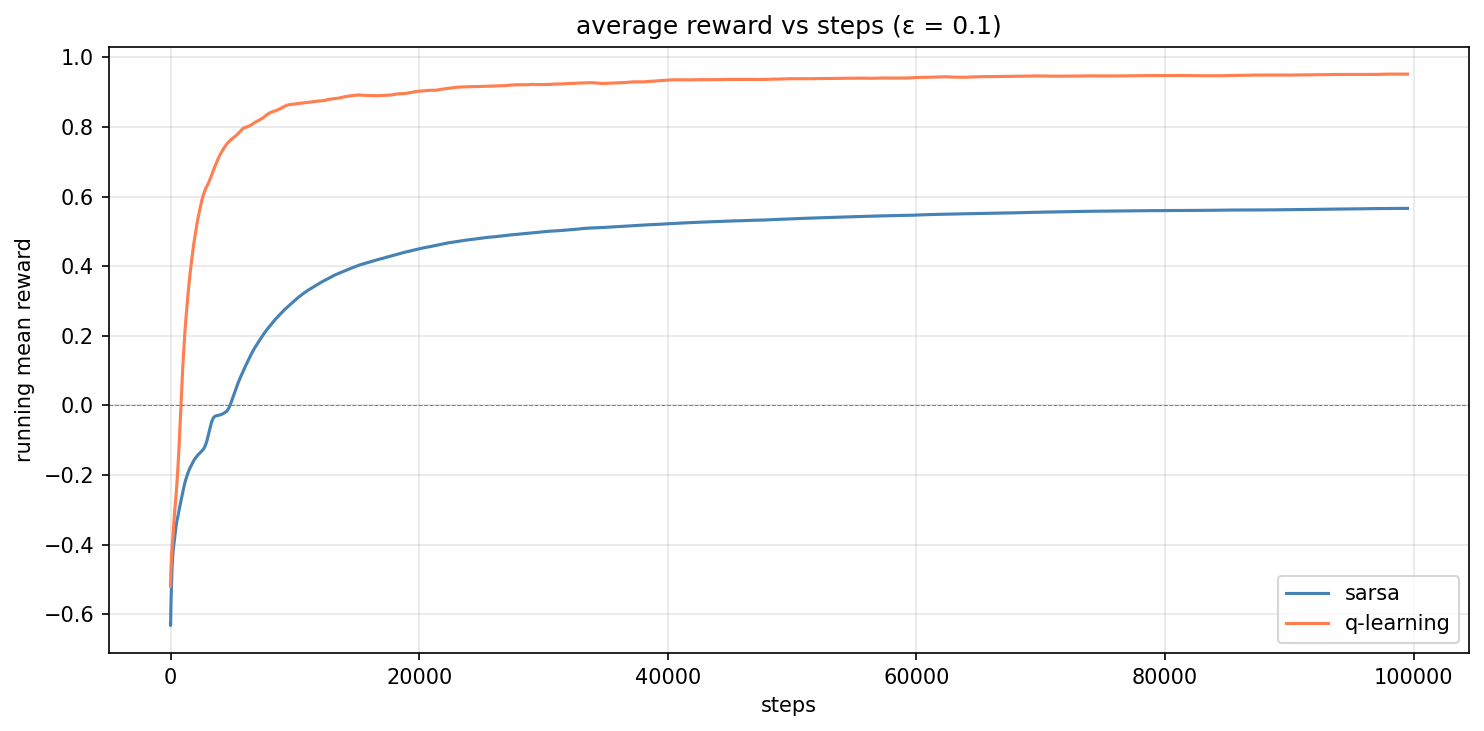
\includegraphics[width=0.75\textwidth]{../02-results/task1_avg_reward.png}
\caption{Running mean reward over 100k steps. SARSA in blue, Q-learning in coral. Smoothed with 500-step window.}
\end{figure}

SARSA got a mean reward of \textbf{0.6373} and Q-learning got \textbf{0.9384}. So Q-learning did better overall. The reason is the max operator --- even when the agent is exploring, the update still chases the best possible action. SARSA learns whatever the agent actually ends up doing, random moves included, so it settles lower.

Both curves shoot up in the first $\sim$10,000 steps as the agents figure out where the goal is, then level off. The wiggles after that are from the 10\% random exploration still going on. The gap between the two lines shows Q-learning pulling ahead over time as its off-policy updates accumulate.

\subsection{Task 2 --- Effect of Epsilon}

\begin{figure}[H]
\centering
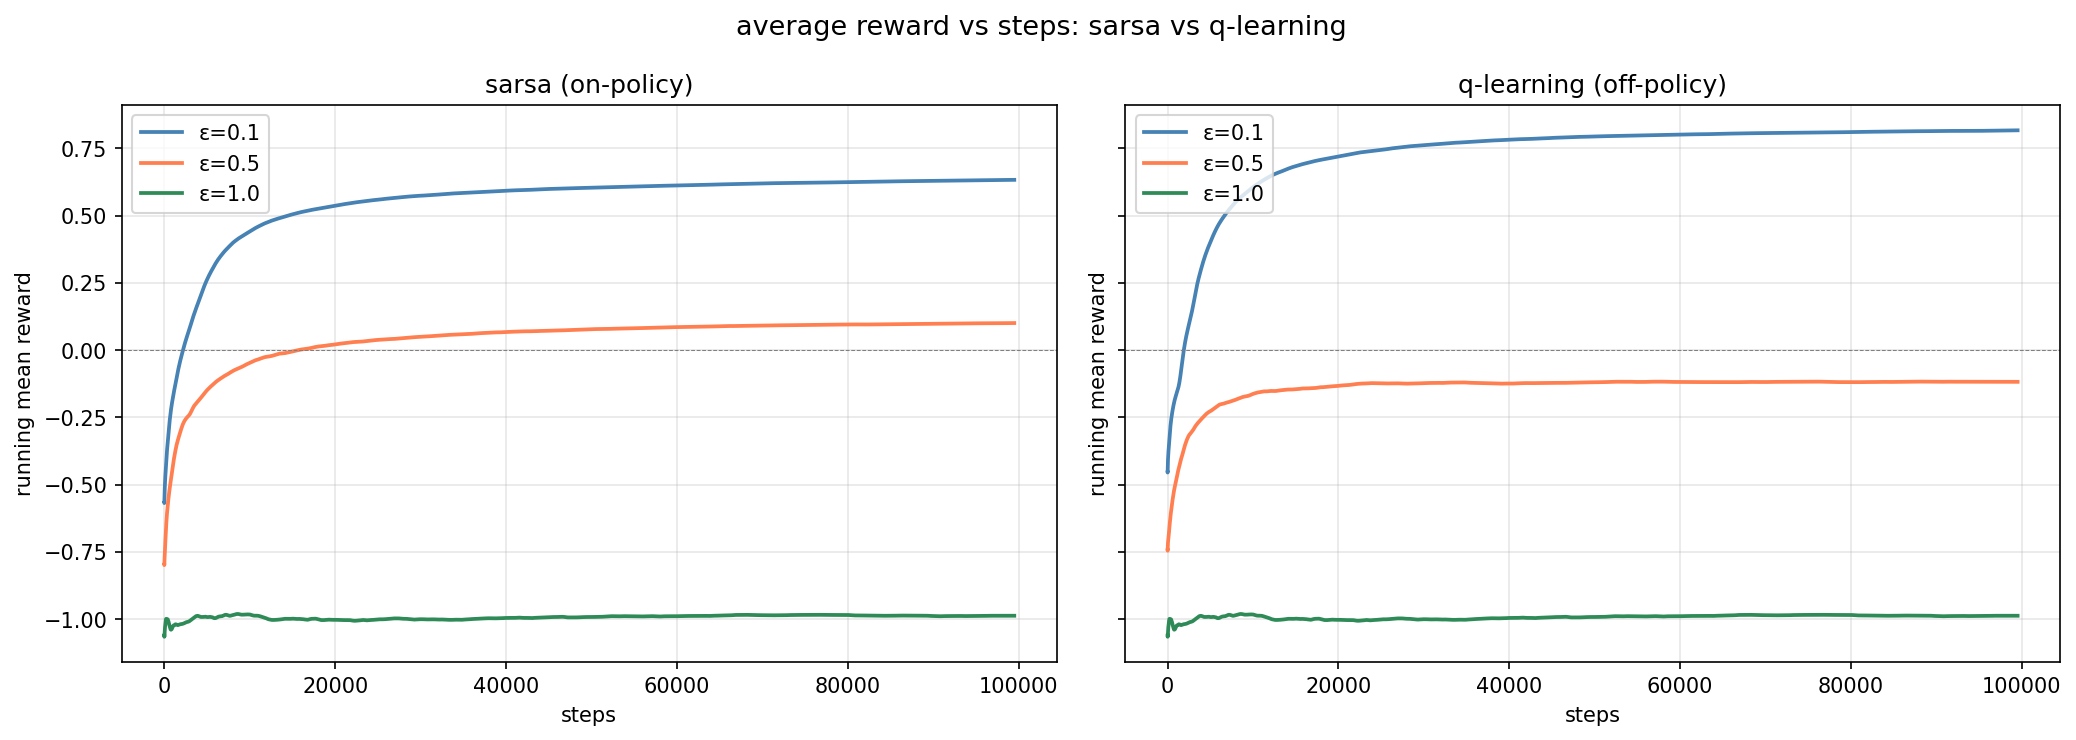
\includegraphics[width=0.85\textwidth]{../02-results/td_epsilon_comparison.png}
\caption{Reward vs steps for SARSA (left) and Q-learning (right) at $\varepsilon = 0.1, 0.5, 1.0$. Averaged over 5 seeds.}
\end{figure}

\begin{figure}[H]
\centering
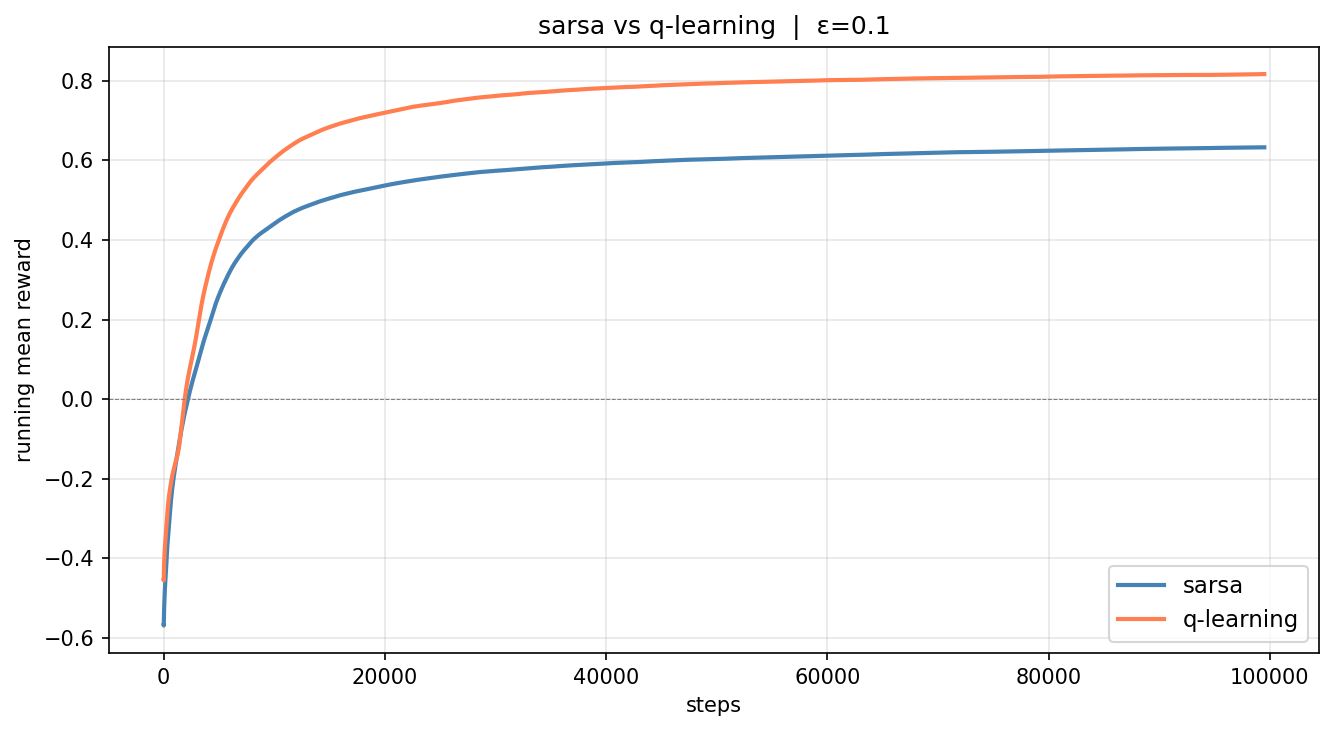
\includegraphics[width=0.75\textwidth]{../02-results/td_sarsa_vs_qlearning.png}
\caption{Direct comparison of SARSA and Q-learning at $\varepsilon = 0.1$.}
\end{figure}

\subsection{Learned Policies}

Both algorithms at $\varepsilon = 0.1$:

\begin{table}[H]
\centering
\begin{tabular}{lcc}
\toprule
Algorithm & Action Values & Greedy Policy \\
\midrule
SARSA &
  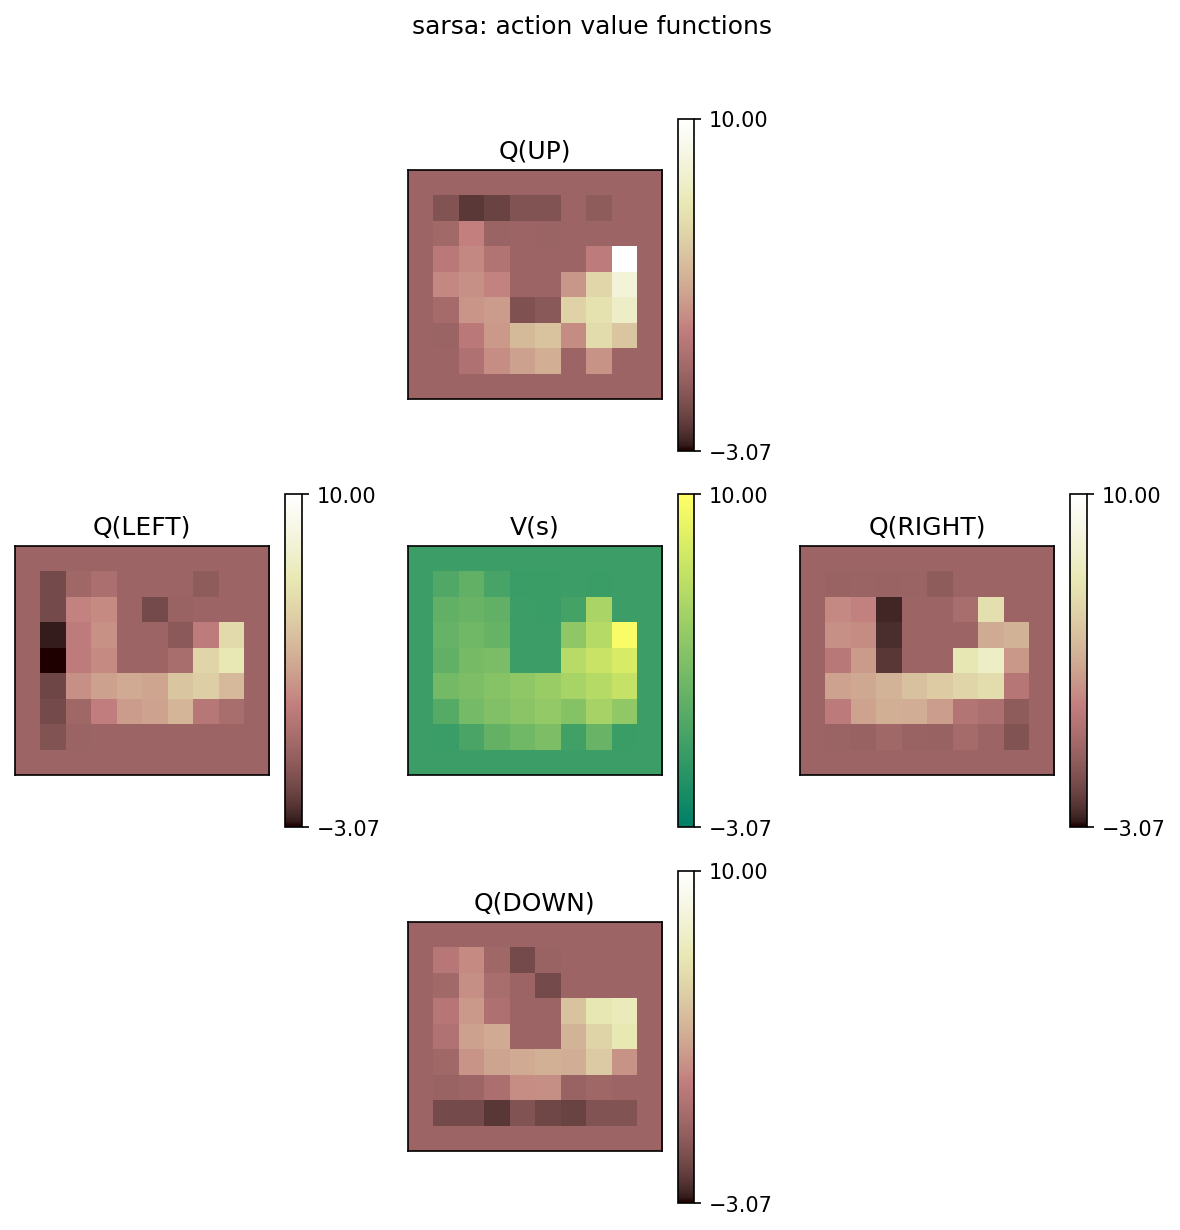
\includegraphics[width=0.3\textwidth]{../02-results/sarsa_q_values.png} &
  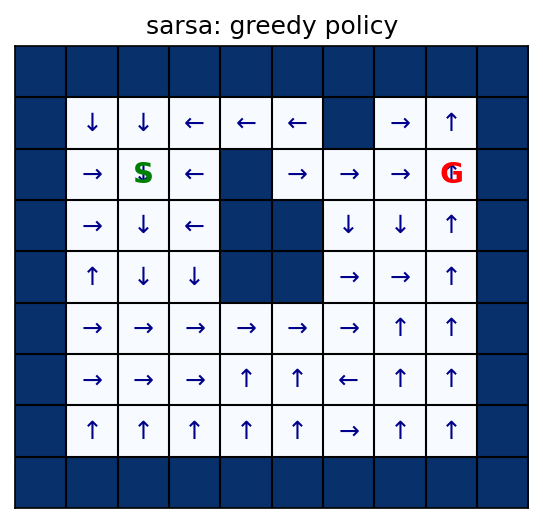
\includegraphics[width=0.22\textwidth]{../02-results/sarsa_policy.png} \\
Q-learning &
  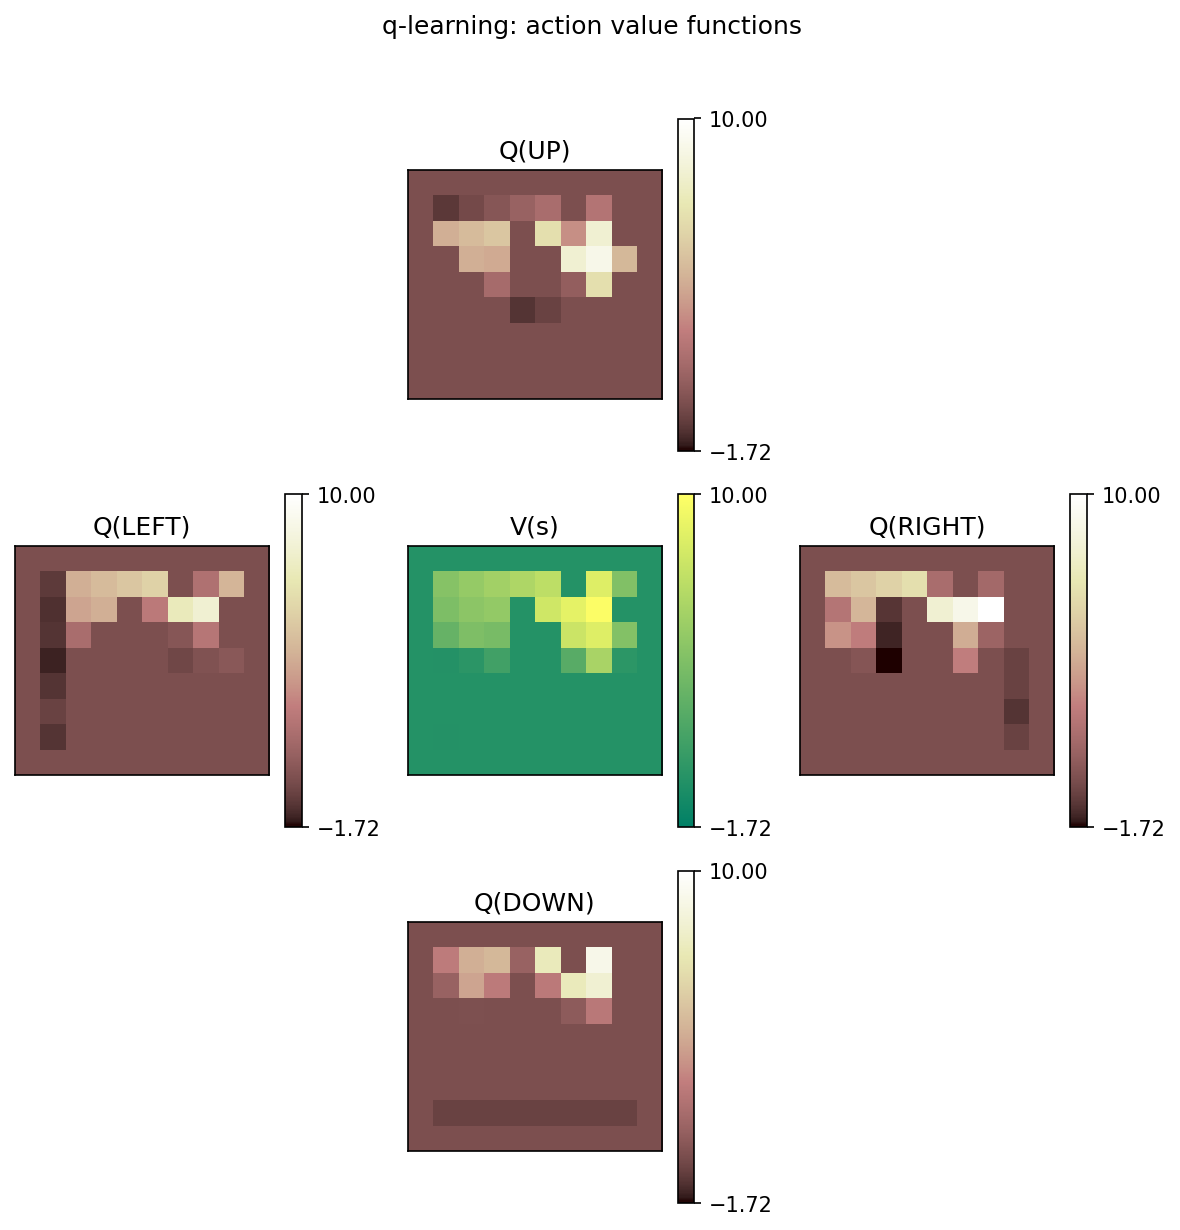
\includegraphics[width=0.3\textwidth]{../02-results/qlearning_q_values.png} &
  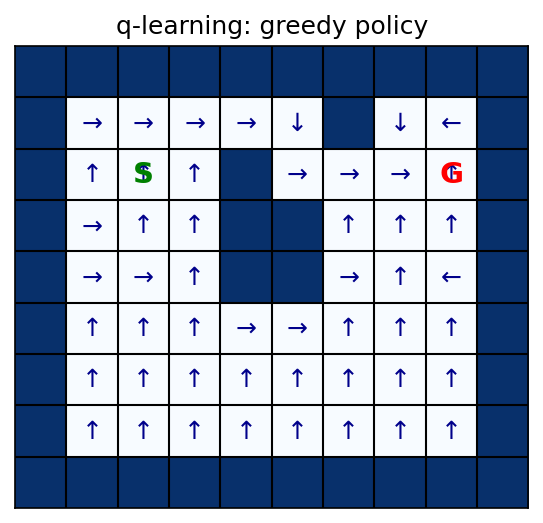
\includegraphics[width=0.22\textwidth]{../02-results/qlearning_policy.png} \\
\bottomrule
\end{tabular}
\end{table}

Both algorithms found decent paths from start to goal going around the walls. The Q-values are highest near the goal and drop off as you move away, which is exactly what TD learning should produce.

% ============================================================
\section{Analysis}
% ============================================================

\subsection{Task 3 --- How Epsilon Affects Training}

\textbf{When $\varepsilon = 0.1$}, both algorithms converge fast and reach the highest average reward. 90\% of the time the agent follows what it knows, so it avoids walls and finds the goal consistently. Q-learning has a slight edge here --- the max operator means it always targets the best action even when exploring. SARSA trails a bit because its update includes whatever random action was taken next, so the noise bleeds into the values.

\textbf{When $\varepsilon = 0.5$}, half the moves are random. Learning slows down a lot and the agent hits way more walls. SARSA suffers more because each update bakes in the random action that just happened --- the noise goes straight into the Q-values. Q-learning resists better since max Q filters out the random action and still tracks the best option.

\textbf{When $\varepsilon = 1.0$}, no learning occurs, and because there are wall penalties and goal rewards, the average reward is near zero and the Q-table is just noise.

More exploration should be good in theory, but in this case will result mainly in more wall penalties. SARSA suffers more from wall penalties since it learns based on a policy that includes all random actions, while Q-learning learns based on policies that do not include the actual outcomes of the random actions.

\subsection{Task 4 --- Optimal Epsilon}

For both algorithms \textbf{$\varepsilon = 0.1$} is optimal.

10\% randomness is enough to give the best chance of finding the goal quickly (all Q's = 0), while 90\% exploitation minimizes wall penalties and maximizes goal rewards.

\textbf{Why not lower?} $\varepsilon = 0$ (all Q = 0) will cause the agent to always pick UP and never attempt any other action, eventually getting stuck in an infinite UP loop.

\textbf{Why not higher?} Increasing $\varepsilon$ after the best path is discovered would result in extra wall penalties for both algorithms and is not beneficial.

While Q-learning does tolerate more noise than SARSA since Q-learning uses max Q for all possible next actions, best trade-off for both algorithms is \textbf{$\varepsilon = 0.1$}.

% ============================================================
\begin{thebibliography}{9}

\bibitem{watkins1992}
Watkins, C.~J.~C.~H. \& Dayan, P. (1992).
Q-learning.
\textit{Machine Learning}, 8(3--4), 279--292.

\end{thebibliography}

\end{document}
